% INTRODUCCIÓN
\chapter{Introducción}

En este capítulo se da una visión general del problema que se ha estudiado así como la motivación para investigar y contribuir en este área. Se explica, también, la relevancia del problema en el marco del procesamiento de imagen y la segmentación. Finalmente, se especifican el propósito y los objetivos que se han guiado esta investigación


% 1.1. MOTIVACIÓN
\section{Motivación}\label{sec:motivacion}

El desarrollo de mecanismos que permiten a las máquinas el aprendizaje de técnicas que les capacitan para la resolución automática de problemas es un campo fundamental dentro del área de la Computación y la Inteligencia Artificial. Este tipo de procesos se utilizan en la vida diaria de muchos seres humanos y resultan innatos en ellos, en cambio, su implementación para que las máquinas los lleven a cabo se convierte en todo un reto debido a la dificultad de la imitación de los procesos cerebrales de las personas.

Muchos autores \cite{lib:ross, lib:boden, art:searle, art:churchland} han propuesto ideas sobre esta cuestión pero debe destacarse a R. Penrose \cite{lib:penrose} que en su libro {\em La nueva mente del Emperador},  se proclama un claro detractor de la idea de que las máquinas puedan llegar a tener la opción de discernir de una forma similar al cerebro humano. Llega incluso a preguntarse ``?`cómo podríamos siquiera {\em empezar} a explicar la substancia de tales problemas a una entidad que no sea ella misma consciente\dots?''

En definitiva, en este trabajo se sustenta en la idea de hacer posible lo que muchos creen imposible, lo que muchos creen que no será posible en mucho tiempo, incluso que no será posible sin conocernos a nosotros mismos. En este sentido, se trata el problema de la segmentación a través de segmentación de imágenes para intentar mejorar los métodos actuales y llegar a un método que pudiera ser utilizado de forma general para cualquier entrada.


% 1.2. DEFINICIÓN
\section{Definición del problema}\label{sec:definicion}
El problema de la segmentación consiste en poder conocer dentro de una imagen qué parte de ella pertenece al objeto u objetos y cual al fondo. Así, por ejemplo, en la figura \ref{img:ejemplomolino} el lector podrá diferenciar claramente el molino del pueblo que se ve en el fondo de la imagen. El hecho de diferenciar un objeto del fondo de una imagen es un proceso que no supone ninguna dificultad para la mente humana; es algo que realizamos inconscientemente cientos de veces durante el día, sin que nos cueste ningún esfuerzo. Sin embargo, la misma tarea puede resultar muy complicada o imposible de realizar a través de un programa informático. Podría ser como aquel hidalgo que veía gigantes en lugar molinos\footnote{En el IV centenario de la publicación de la segunda parte de ``El Quijote''.}.

\begin{figure}
	\centering
	\includegraphics[width=0.45\textwidth]{img/molino.jpg}
	\caption{Distinguir el molino del pueblo del fondo no es difícil para un humano aunque sí para una máquina.}
	\label{img:ejemplomolino}
\end{figure}

%\REV{pq es importante el problema de la segmentación} 
Este problema tiene una especial importante en la automatización de tareas, como el reconocimiento de direcciones postales, el realzamiento de textos o sistemas de calidad en grandes industrias, por ejemplo. También se utiliza en campos tan importantes como la medicina para poder ver en tiempo real la situación del tumor de un paciente. En definitiva, es importante ya que hace que un programa pueda tener como entrada una imagen en vez de valores discretos y obtener otra imagen que nos da muchísima información de la primera y que es facilmente interpretable por personas y más sencilla para las máquinas.

Autores como González y Woods \cite{lib:gonzalez} enuncian el problema de ``segmentación de imágenes no triviales como una de las tareas más dificiles en el procesamiento de imágenes''. En este sentido, insisten en que ``la exactitud de la segmentación determina el éxito o error de los procesos de análisis computerizados''. Otros autores \cite{lib:sonka} hablan de la sementación como una ``técnica en al que se divide la imagen en partes que tienen una correlación con objetos o áreas del mundo real contenidas en la imagen''.

\begin{definition}\label{def:definicionproblema}
Dada una imagen $Q$ que se puede subdividir en $n$ regiones $R_{1}, \dots, R_{n}$, y conocida $P$ que es una cierta propiedad booleana que cumplen todos los píxeles de la región $R_{i}, \forall  i=1,\dots ,n$, se deberá cumplir siempre que:
\begin{enumerate}
	\item $\bigcup_{i=1}^{n}R_{i}=Q$;
	\item En una región $R_{i}, \forall i=1,\dots ,n$ todos sus píxeles están conectados;
	\item $R_{i}\cap R_{j}=\emptyset, \forall i, j : i\neq j;$
	\item $P(R_{i}) = \text{ VERDADERO }, \forall  i=1,\dots ,n;$
	\item $P(R_{i}\cup R_{j}) = \text{ FALSO }, \forall  i=1,\dots ,n.$
\end{enumerate}
\end{definition}

Se hablará de segmentación monoumbral cuando se obtenga únicamente un objeto y el fondo con un único umbral $t$. Para más de un objeto se dirá que el problema es multiumbral, con un vector de umbrales $(t_1, \dots, t_{n-1})$.

En conclusión, en este proceso se lleva a cabo la división de la imagen en regiones donde cada una (desde 2 hasta $n$, este número dependerá del problema que estemos resolviendo) harán mención al fondo y a cada objeto. Además, todas las regiones serán independientes entre sí, esto es, un pixel pertenecerá solamente a la región $i$ cuando hablemos de segmentación completa. Centrando el problema únicamente en aquellas imágenes en escala de grises, nuestra pretensión será obtener aquellas regiones que contienen a un objeto a través de su histograma (frecuencia de los tonos de gris), esto es, por medio de técnicas de umbralización. %\REV{seguro?}. Hablado del tema del gris con histograma


% 1.3. SOLUCIÓN
\section{Solución propuesta}\label{sec:solucion}
%\REV{Nosotros vamos a utilizar técnicas difusas, para empezar. ¿Por qué? (Incertidumebre en torno a los píxeles, péridda de información captación imágenes,...)}

Para llevar a cabo este estudio se ha utilizado la representación de las imágenes por medio de conjuntos difusos. Estas técnicas, en comparación con las habituales de lógica clásica, consiguen evitar que haya perdida de información en las imágenes. Esto se debe a que en la obtención y discretización de las imágenes se llevan a cabo simplificaciones sobre la definición real con intención de poder ser representado digitalmente. 

Asimismo, la incertidubre que puede haber en torno a los problemas relacionados con el procesamiento de imagen es alto. En particular, la segmentación busca separar de forma excluyente los objetos del fondo, algo que se hace imposible de definir de forma certera. Se conoce que en un cambio de intensidad suficientemente fuerte estará un borde pero, justamente, por el hecho de que el propio enunciado sea de por sí difuso (suficientemente fuerte), será necesario poder representar esta incertidumbre, algo que haremos por medio de los conjuntos que definió Zadeh.

Además, existen tres técnicas para poder llevar a cabo la segmentación de una imagen \cite{lib:gonzalez}:
%\REV{explicación y referencia}
\begin{enumerate}[label=\alph*)]
	\item {\em Segmentación basada en umbralización}. A través de uno o varios umbrales se obtiene una forma de clasificar todos los píxeles de la imagen en una única región buscando que las regiones tengan un cierto significado. 
	\item {\em Técnicas basada en agrupamiento de píxeles en regiones}. Se procede clasificando cada uno de los píxeles de la imagen dentro de las regiones buscando que estas se creen con los píxeles más similares. Se suele indicar el número de regiones que se desea obtener.
	\item {\em Técnicas basadas en la detección de bordes}. Basan su técnica en la identificación de los píxeles en la frontera. Se detecta el objeto y el fondo, ya que de esta forma queda definido también su contorno.
\end{enumerate}

En este trabajo se va a centrar la segmentación por medio de las técnicas de umbralización. Para ello lo que tendremos que hacer será calcular los umbrales que separen las regiones que se hayan encontrado, de forma que situaremos las regiones entre un umbral $t_{i}$ y otro $t_{i+1}$. Para ejemplificar esto, tomaremos la umbralización binaria en la cual se dispondrá de un único umbral $t$. De esta forma, todos los elementos de la imagen que se encuentren por encima del umbral pertenecerán a una región  y los que estén por debajo a la segunda. Esta técnica se basa únicamente en detectar los diferentes tonos de gris de la imagen, así que mirando el histograma de la imagen (fig. \ref{img:rice}), podríamos ver cómo existe una frontera entre la intensidad $t=71$ y el resto creando diferencias en los niveles de gris. \cite{art:refbarrenechea}

\begin{figure}
\centering
	\subfigure[Imagen original.]
	{\includegraphics[width=0.25\textwidth]{img/rice}}\quad
	\subfigure[Imagen segmentada.]
	{\includegraphics[width=0.25\textwidth]{img/umbra-rice}}\quad
	\subfigure[Histograma.]
	{\includegraphics[width=0.35\textwidth]{img/hist-rice}}
	\caption{Proceso de segmentación. Se puede ver que en $t=71$ se produce un mínimo con respecto a los otros niveles de gris y que por eso se escoge como umbral.}
	\label{img:rice}
\end{figure}


%\REV{solución al pq...} Escrita
Se debe tener en cuenta que la umbralización es un método rápido y de coste computacional bajo por lo que se puede realizar en tiempo real. Como sólo basa su algorítmica en el histograma de la imagen hace que sea un método sencillo e intuitivo, aunque esto también hace que tenga problemas ante el ruido y objetos o fondos que no sean uniformes.

La solución que se presenta en este trabajo se obtiene por medio de lógica difusa. Se han utilizado funciones REF, de Dombi, de agregación y penalti. En el capítulo \ref{basicos} se hace mención a todos estos conceptos y se explican poníendose en práctica a partir del capítulo \ref{monoumbral}. En el capítulo \ref{cap:conclusiones} se presentan todas las conclusiones obtenidas así como las líneas de trabajo futuro.

%La umbralización es rápida, de coste computacional bajo y se puede realizar en tiempo real.
%Sencilla e intuitiva.
%Técnica útili si el fondo y los objetos son uniformes.
%Problemas: el ruido, niveles de gris similares entre obejto y fondo, solapamientos de objetos...
%La obtención de un umbral se basará en el histograma de la imagen. No se considera la información espacial.

% 1.4. REELEVANCIA
\section{Relevancia}\label{sec:relevancia}

En el campo de la medicina \cite{lib:suri, lib:sonka} se ha experimentado una mejora sustancial en la efectividad de las pruebas médicas gracias a diferentes opciones como los rayos X, la tomografía computerizada, la resonancia magnética, la tomografía por emisión de positrones (PET), imágenes de ultrasonidos y otras. La revolución digital y el gran poder de procesamiento que disponen los ordenadores ha conseguido que los profesionales comprendan la compleja anatomía humana, aunque esto no ha sido suficiente ya que se ha visto necesario poder obtener los bordes, las superficies y la segmentación de los órganos. Estos órganos segmentados y sus bordes son clave para poder conseguir que un especialista médico pueda hacer una cirugía adecuada para muchas ramas de la medicina, debido a la importancia de tener datos en tiempo real \cite{url:noticiasegmentacion}. %\REV{[Insertar figura que vaya con esto].}
\begin{figure}
\centering
	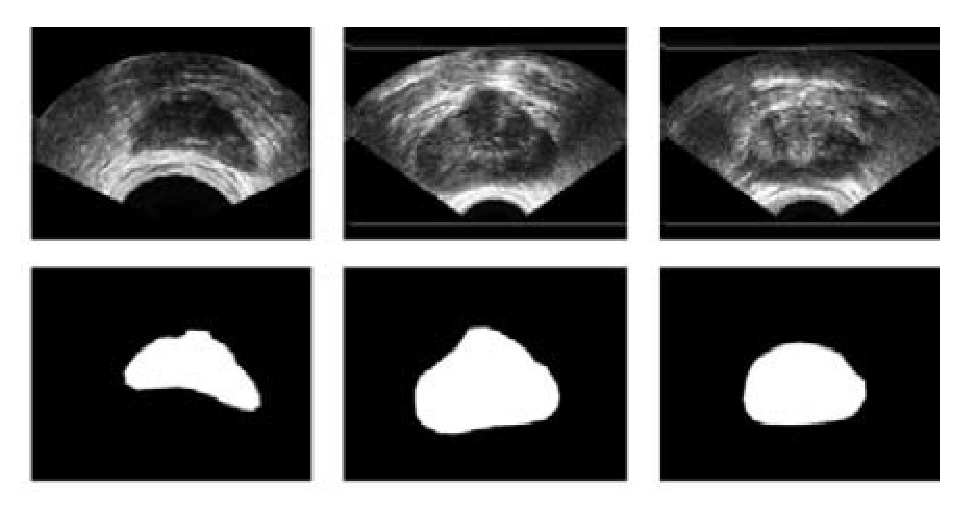
\includegraphics[width=0.5\textwidth]{img/imagenmedica.eps}
	\caption{Segmentación de una imagen de próstata \cite{art:bustincesegmedica}.}
	\label{img:segmentacionmedica}
\end{figure}

%Pruebas médicas
%Localización de tumores y otras patologías
%Medida de volúmenes de tejido
%Cirugía guiada por ordenador
%Diagnóstico
%Planificación del tratamiento
%Estudio de la estructura anatómica

Por otra parte, en los sistemas de seguridad hoy en día se utilizan factores biométricos como clave. Un claro ejemplo es el uso de la huella dactilar. En este sentido, antes de llevar a cabo el reconocimiento de la huella se hace imprescindible aplicarle la segmentación para poder obtener la mayor información posible de la huella. Se utiliza también la segmentación en procesos de calidad, sobre todo de cadenas de producción, donde todos los productos de salida son iguales. En este caso, será sencillo detectar diferencias entre la salida adecuada y la defectuosa para poder retirarla. Esto se generaliza en la detección de errores en diferentes campos de la industria y la sociedad.

\begin{figure}
\centering
	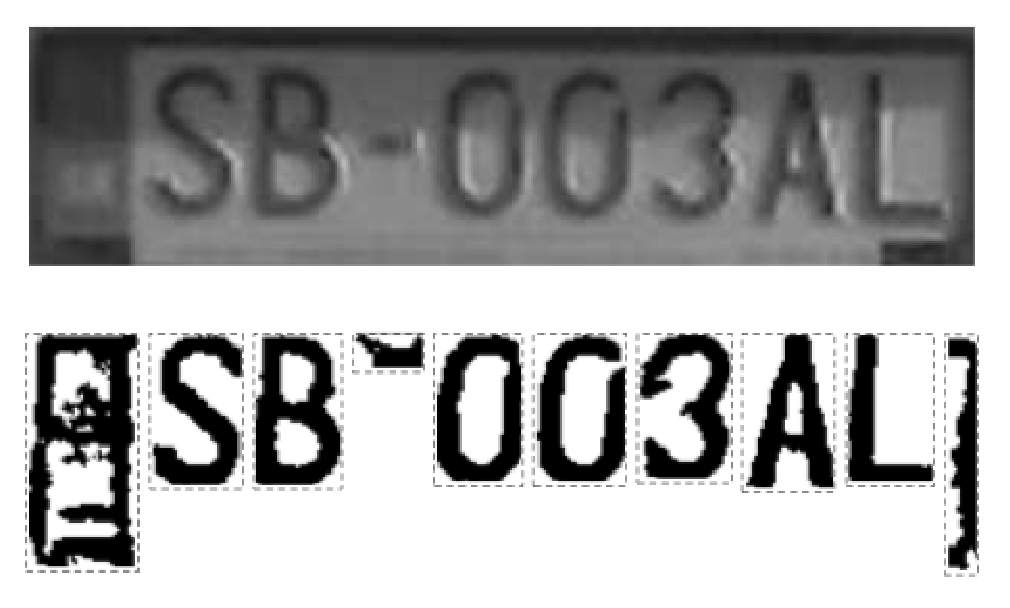
\includegraphics[width=0.4\textwidth]{img/matricula.eps}
	\caption{Utilización de técnicas de segmentación para extraer la información de una matrícula y poder ser procesada por un sistema de IA.\cite{lib:matricula}.}
	\label{img:matricula}
\end{figure}

En definitiva, el problema de la segmentación de la imagen se hace importante ya que busca que la entrada del problema no sean datos concretos sino imágenes que después se interpretarán. Para que esta interpretación se correcta, el poder disponer de una información certera, sencilla y limpia se hace fundamental.

%Análisis automático de detección de errores.

%Sensor de huella digital
%Localización de objetos en imágenes de satélite (teledetección).
%\REV{Alargar esto}


% 1.5. OBJETIVOS
\section{Propósito y objetivos}\label{sec:objetivos}

Este proyecto se centra en estudiar técnicas de segmentación para un único umbral en imágenes en blanco y negro e intentar mejorar las técnicas de las que actualmente se disponen intentando generalizarlas de forma que los parámetros no dependan del problema. 

Además, para poder conseguir el propósito anterior se estipularon los siguiente objetivos:
\begin{itemize}
	\item Investigar y conocer técnicas actuales de segmentación de imagen de forma que estas sean el punto de partida.
	\item Analizar y evaluar las funciones que J. Dombi propone en \cite{art:dombi}. Comparar estas con las funciones REF y sustituirlas en la construcción de los conjuntos difusos para conocer sus efectos.
	\item Implementar diferentes algoritmos de segmentación con el conocimiento adquirido anteriormente evaluando su mejora y haciendo las correcciones necesarias con la intención de generalizar el método de forma máxima.
	\item Dirimir cual es el mejor umbral a través de la agregación de resultados y obtención del mejor con funciones penalti.
	\item Implementar diferentes algoritmos que incluyan la agregación OWA de las diferentes funciones estudiadas para la segmentación en los puntos anteriores comprobando si esto mejora los resultados anteriores.
	\item Analizar todos los puntos anteriores a fin de concluir los resultados del trabajo así como dirimir si se ha podido conseguir cumplir el propósito inicial.
\end{itemize}
